% =====================================================================
%  Informe divulgativo para el director de tesis
%  Compilar: pdflatex informe_director.tex  (dos veces)
%  o arrastrar la carpeta a Overleaf.
% =====================================================================
\documentclass[11pt,a4paper]{article}

\usepackage[utf8]{inputenc}
\usepackage[T1]{fontenc}
\usepackage[spanish,es-tabla]{babel}
\usepackage{lmodern}
\usepackage{microtype}
\usepackage{amsmath,amssymb}
\usepackage{booktabs}
\usepackage{graphicx}
\usepackage{siunitx}
\usepackage{caption}
\usepackage{float}
\usepackage[margin=2.5cm]{geometry}
\usepackage{setspace}
\usepackage{fancyhdr}
\usepackage{xcolor}
\usepackage{mdframed}
\usepackage[colorlinks=true,linkcolor=black,citecolor=black,urlcolor=blue]{hyperref}

\sisetup{output-decimal-marker = {.}, group-separator = {\,}}
\graphicspath{{figuras_informe/}}
\onehalfspacing
\captionsetup{font=small,labelfont=bf}

\pagestyle{fancy}
\fancyhf{}
\fancyhead[L]{\small Imputación de señales SiPM --- Informe de resultados}
\fancyhead[R]{\small\thepage}
\renewcommand{\headrulewidth}{0.4pt}

% Recuadro para las ideas que hay que retener
\definecolor{cajafondo}{RGB}{240,244,248}
\definecolor{cajaborde}{RGB}{70,110,150}
\newmdenv[backgroundcolor=cajafondo,linecolor=cajaborde,linewidth=1.2pt,
          leftmargin=0pt,rightmargin=0pt,innertopmargin=8pt,
          innerbottommargin=8pt,skipabove=10pt,skipbelow=10pt]{idea}

\title{\vspace{-1.5cm}\textbf{Recuperación de sensores averiados en un detector PET
de cristal monolítico}\\[0.3cm]
\large Informe de resultados y guía de lectura de las figuras}
\author{Miguel Escudero}
\date{Agosto de 2026}

\begin{document}
\maketitle
\thispagestyle{fancy}

\begin{idea}
\noindent\textbf{En dos frases.} Una red neuronal que explota la geometría hexagonal del
detector reconstruye la carga de un sensor averiado a partir de los sesenta restantes, y
recupera algo más de la mitad del error de posición que introduce el fallo, conservando
además el espectro de energía y mejorando la resolución espacial. El rendimiento no
depende del tamaño de la red ni de la sofisticación de la arquitectura ---nueve estrategias
distintas no lo mueven---, sino del límite de información que físicamente queda en los
sensores supervivientes.
\end{idea}

\section{Qué problema se resuelve y por qué tiene solución}

El detector es un cristal centelleador monolítico leído por \textbf{61 fotosensores SiPM}
dispuestos en una retícula hexagonal. Cuando un fotón gamma interactúa en el cristal, la luz
producida se reparte entre varios sensores, y la posición del impacto se reconstruye como
un centro de gravedad de las cargas medidas. Si un sensor se avería, su carga desaparece del
cálculo, el centro de gravedad se desplaza y la posición reconstruida queda sistemáticamente
sesgada. El módulo entero deja de ser utilizable.

La propuesta consiste en \textbf{estimar la carga que habría registrado el sensor averiado}
a partir de los sesenta que siguen funcionando, de modo que el cálculo de la posición pueda
completarse. Que esto sea posible no es evidente a priori, y conviene justificarlo: la luz
de centelleo no cae sobre un único fotosensor sino que se reparte sobre una vecindad, de
manera que la información de cada sensor está \textbf{parcialmente contenida en los que lo
rodean}. Esa redundancia es lo que hace viable la reconstrucción. Y es una redundancia
\emph{local}: el tratamiento superficial del cristal confina la luz, así que son los vecinos
inmediatos los que llevan la información, no el detector entero.

El entrenamiento es \textbf{auto-supervisado}. En un módulo realmente averiado la carga
verdadera del sensor muerto es inobservable, así que no existen ejemplos etiquetados. Lo que
sí hay son 159 módulos sanos: en ellos se apaga artificialmente un sensor, se le pide a la
red que lo reconstruya, y su valor real ---que sí conocemos--- sirve de respuesta correcta.

\begin{figure}[H]
\centering
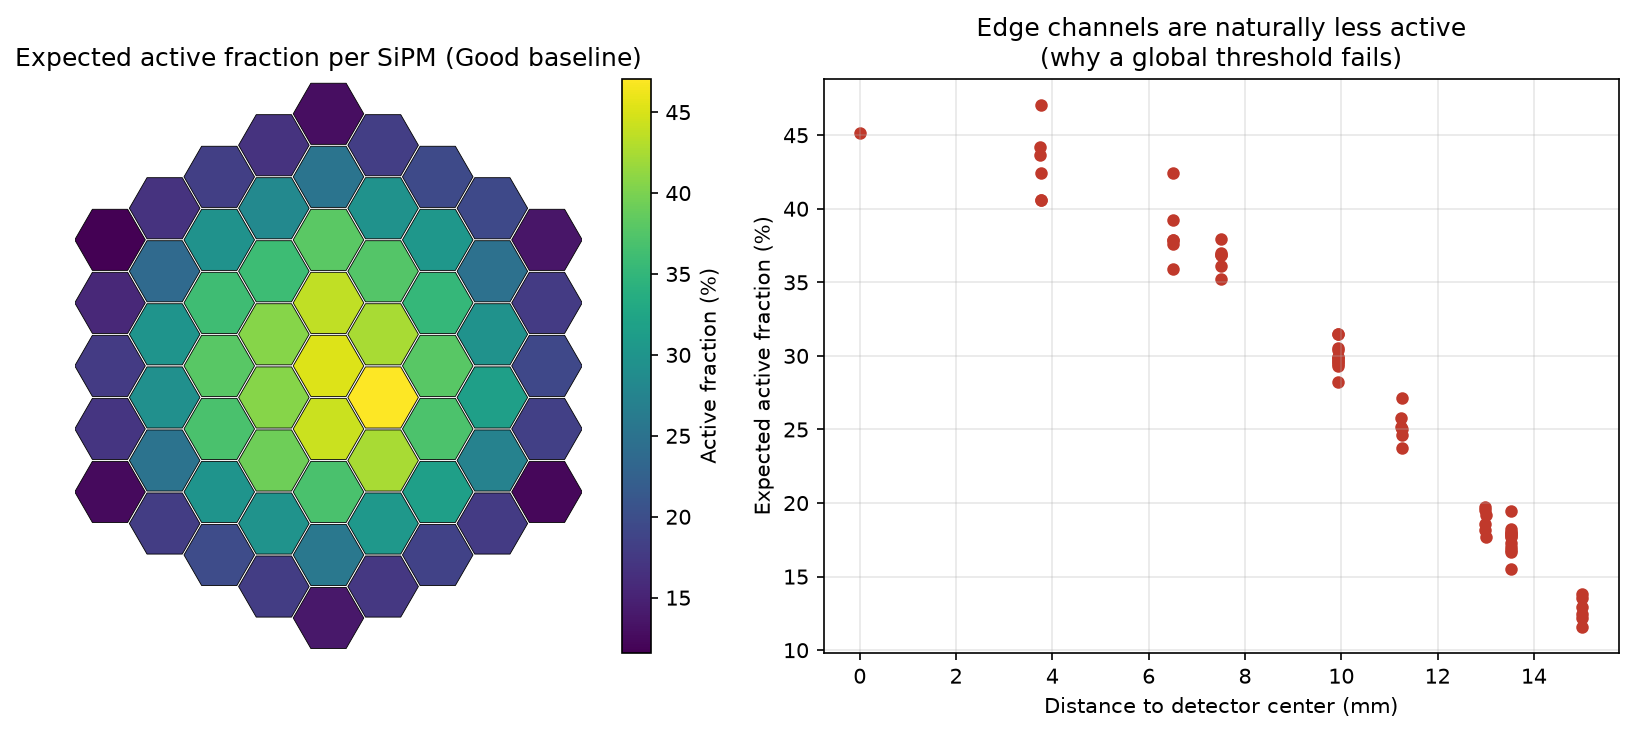
\includegraphics[width=\textwidth]{fig-detector.png}
\caption{\textbf{Geometría del detector y su gradiente natural.} A la izquierda, los 61
sensores dibujados en su posición física real; el color indica la fracción de eventos en
los que cada sensor registra señal, desde el violeta oscuro (en torno al 12\,\%) hasta el
amarillo (cerca del 47\,\%). Se aprecia que \textbf{los sensores centrales se activan mucho
más a menudo que los de las esquinas}. A la derecha, ese mismo dato representado frente a la
distancia al centro del detector: cada punto rojo es un sensor, y la caída es
prácticamente monótona. La causa es física: las caras laterales del cristal llevan un
adhesivo absorbente que suprime las reflexiones, de modo que en el borde se recoge menos
luz. Esta figura conviene tenerla presente porque explica por qué los sensores periféricos
son sistemáticamente más difíciles de reconstruir.}
\label{fig:detector}
\end{figure}

\section{El resultado, visto de un vistazo}

Antes de entrar en métricas conviene mirar el efecto sobre la imagen que se usa a diario en
el laboratorio: el \emph{flood map}, el histograma bidimensional de las posiciones
reconstruidas. En un detector sano dibuja una retícula regular de puntos, uno por cada
sensor.

\begin{figure}[H]
\centering
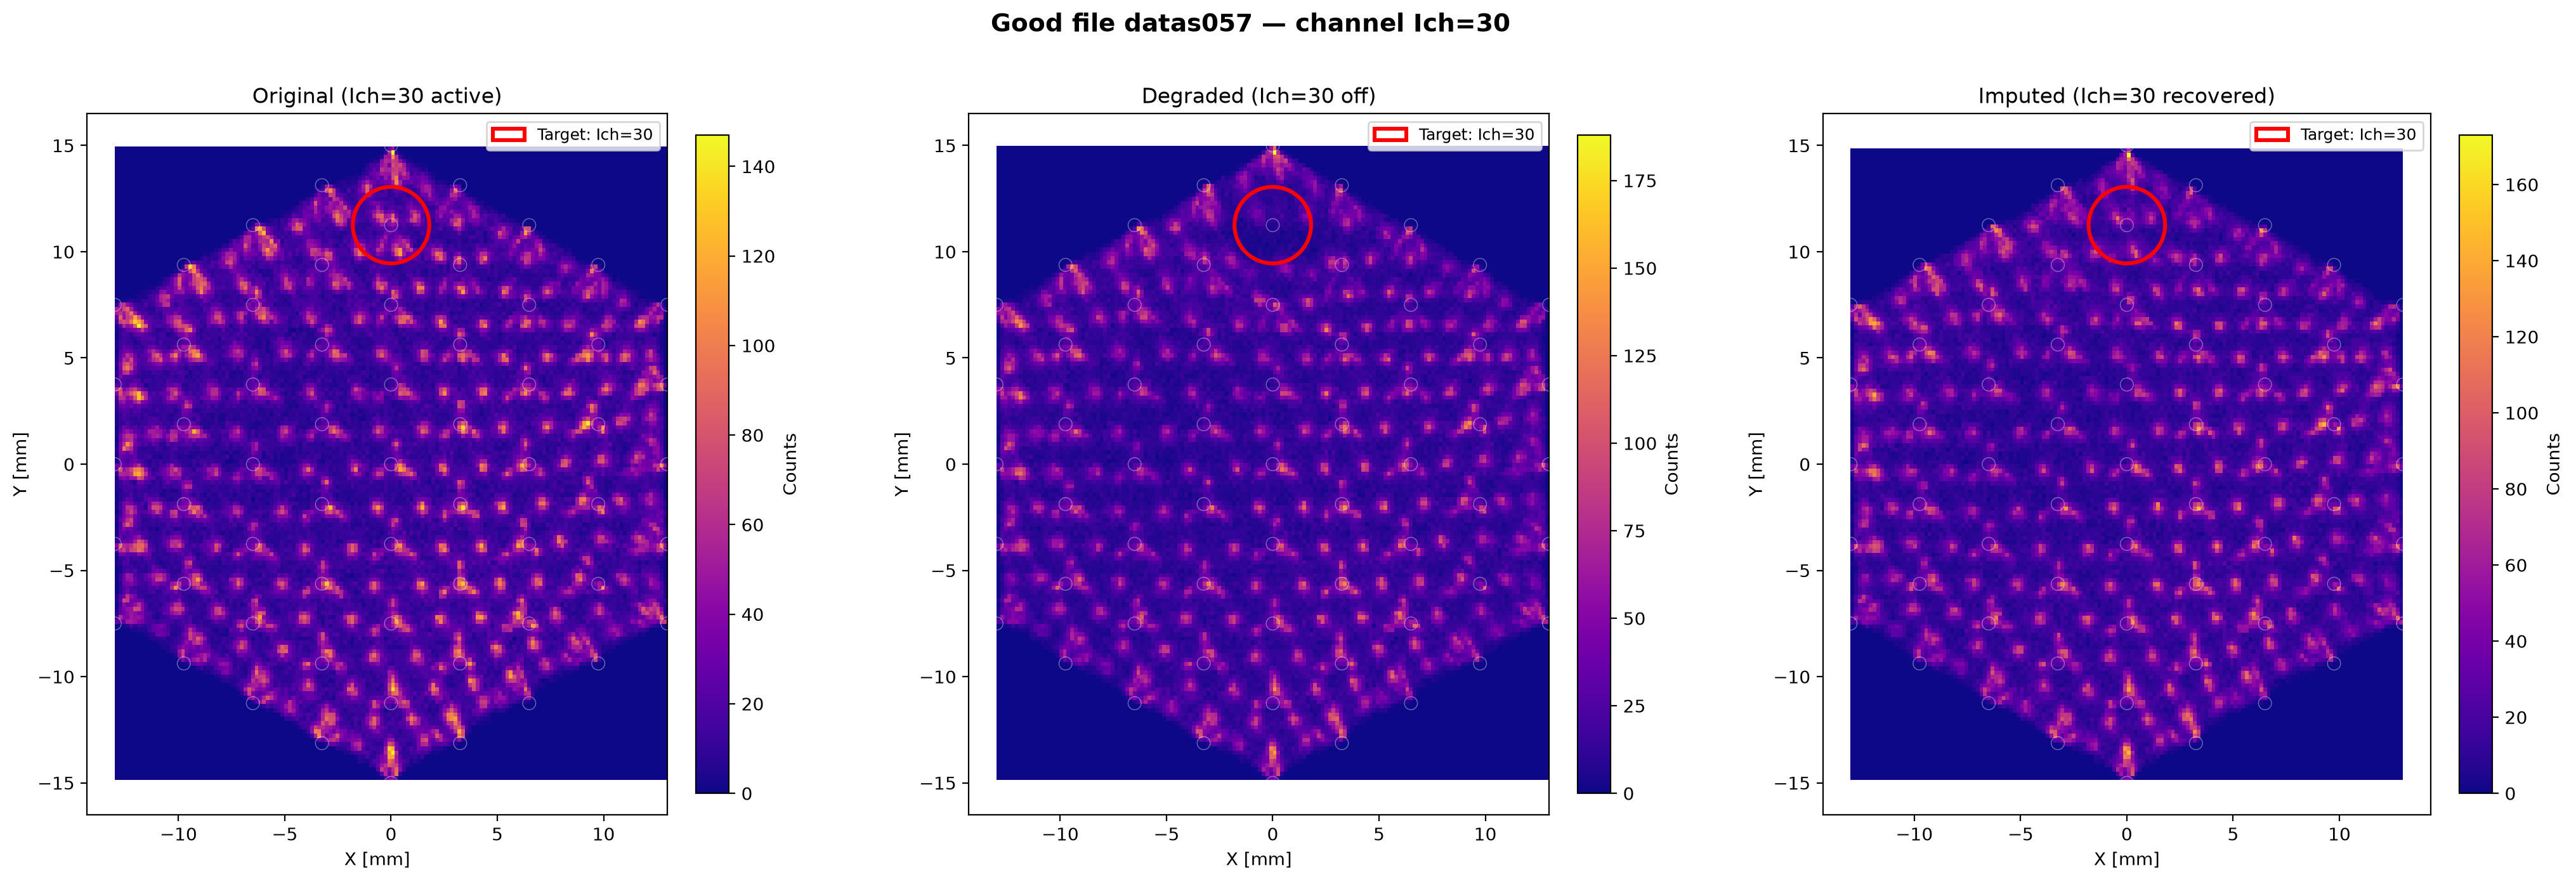
\includegraphics[width=\textwidth]{fig-floodmap.png}
\caption{\textbf{El problema y su corrección, sobre el flood map.} Los tres paneles muestran
el mismo módulo y los mismos eventos. El \textbf{panel izquierdo} es la situación normal,
con los 61 sensores operativos: la retícula de puntos brillantes aparece completa y regular.
El \textbf{panel central} muestra qué ocurre al apagar el sensor \texttt{Ich\,30}: dentro
del círculo rojo la retícula se deforma y aparece un hueco, porque los eventos que ocurrían
en esa zona se reconstruyen ahora en posiciones equivocadas. El \textbf{panel derecho} es el
resultado tras reconstruir la carga del sensor con la red: \textbf{la retícula se recompone}
y el hueco desaparece. La escala de color indica el número de cuentas en cada píxel, de azul
oscuro (ninguna) a amarillo (máximo).}
\label{fig:floodmap}
\end{figure}

\subsection{Cómo se mide, en cristiano}

Todo el trabajo se apoya en una única cantidad: el \textbf{desplazamiento de la posición
reconstruida}, que llamamos $\Delta R$ y medimos en milímetros. Para cada evento se calcula
la posición con los 61 sensores (la verdad), después con el sensor apagado (el fallo), y por
último con el sensor reconstruido por la red. La comparación entre la segunda y la tercera
dice cuánto del daño se ha reparado.

De ahí sale la \textbf{recuperación}, expresada en tanto por ciento: si el fallo desplazaba
la posición un milímetro y tras la reconstrucción se desplaza medio, la recuperación es del
50\,\%. El 100\,\% significaría reconstrucción perfecta y el 0\,\% que la red no aporta
nada. Un valor \emph{negativo} ---que aparecerá más adelante--- significa que la
reconstrucción empeora la posición respecto a no hacer nada.

Se reportan dos versiones de esa cantidad, y merece la pena distinguirlas porque aparecen en
todas las tablas. La \textbf{recuperación media} promedia sobre todos los eventos y es la
cifra honesta, la que resume el comportamiento global. La \textbf{recuperación p90} se fija
en el percentil 90 de la distribución, es decir, en el 10\,\% de eventos peores: describe el
régimen desfavorable, que es el que estropea la imagen.

\begin{idea}
\noindent\textbf{Cifra principal.} Con un sensor averiado, la red recupera de media el
\textbf{50.8 $\pm$ 2.2\,\%} del desplazamiento de posición, y el
\textbf{56.6 $\pm$ 2.3\,\%} en el 10\,\% de eventos peores. El modelo tiene
\textbf{38\,305 parámetros}, un tamaño muy modesto.

\smallskip
\noindent Las barras no son un detalle menor y conviene explicar de dónde salen: proceden de
repetir todo el procedimiento con \textbf{cinco particiones distintas} de los datos, cada una
reservando cinco detectores diferentes para la evaluación final. La dispersión entre ellas es
la incertidumbre real de la cifra, y resulta ser unas veinte veces mayor que la debida a
repetir el entrenamiento. Se detalla en la Sección~\ref{sec:variabilidad}.
\end{idea}

\begin{figure}[H]
\centering
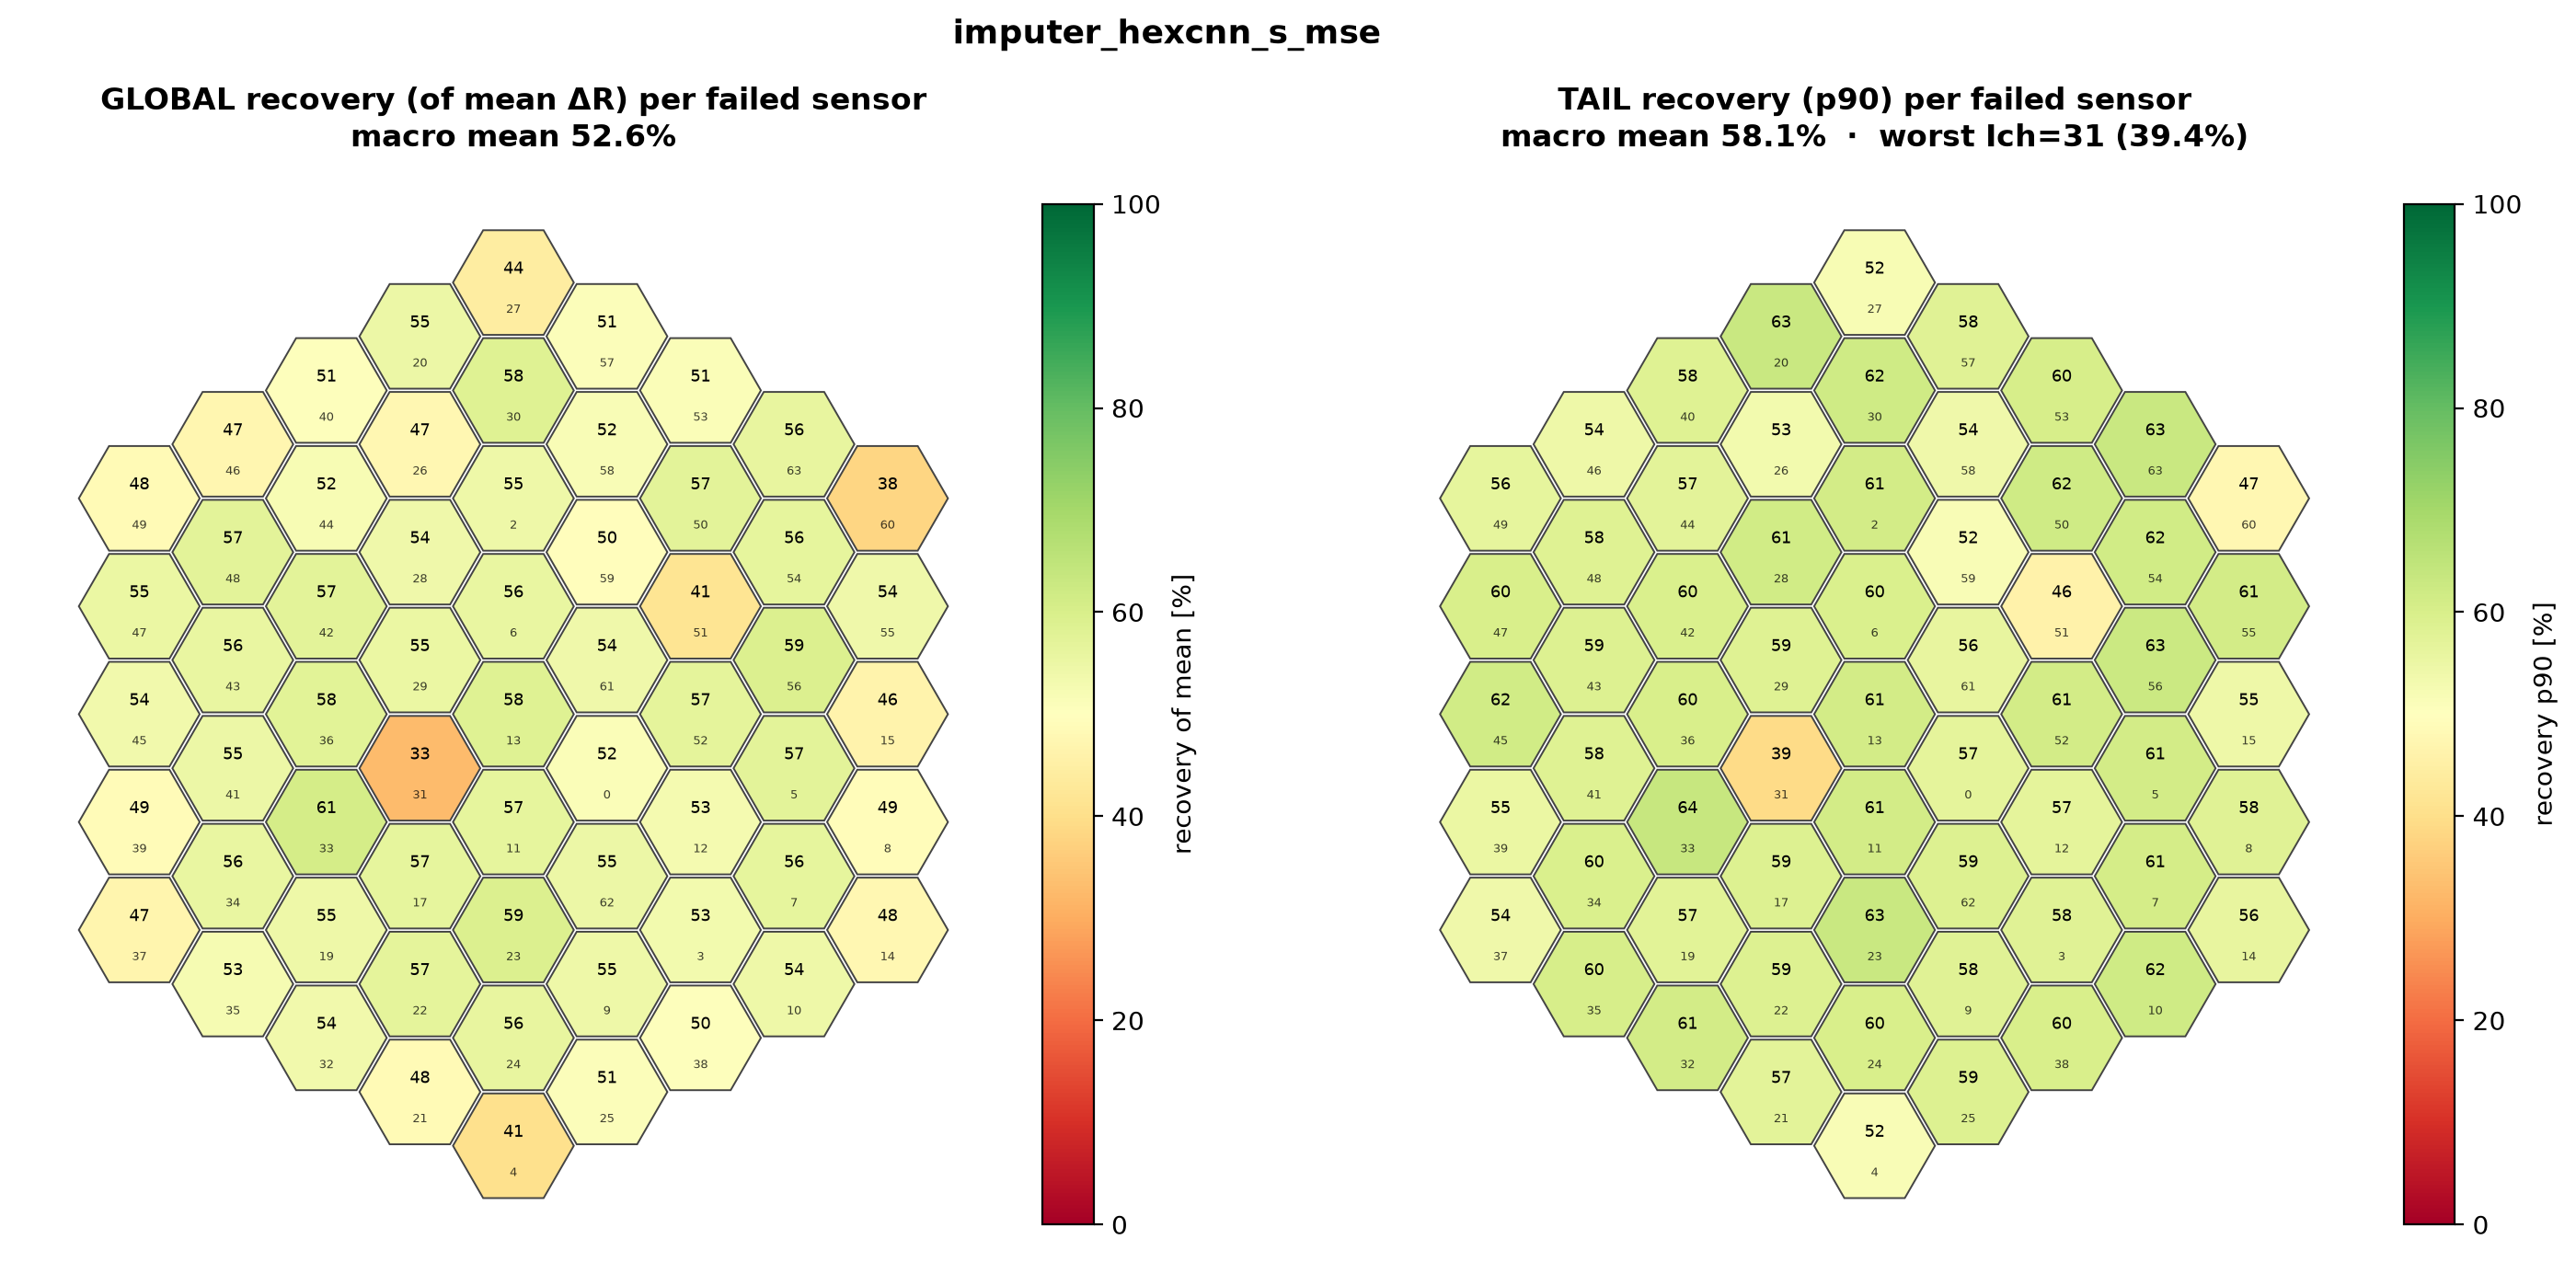
\includegraphics[width=\textwidth]{fig-mapa-recuperacion.png}
\caption{\textbf{Recuperación sensor a sensor.} El experimento se repite apagando cada uno
de los 61 sensores por separado. Cada hexágono representa un sensor en su posición real; el
número grande es el porcentaje recuperado cuando \emph{ese} sensor es el averiado, y el
número pequeño de debajo es su identificador. La escala de color va de rojo (recuperación
nula) a verde (recuperación total), pasando por amarillo en torno al 50\,\%. El
\textbf{panel izquierdo} muestra la recuperación media y el \textbf{panel derecho} la del
10\,\% de eventos peores. La lectura importante es que \textbf{el color es homogéneo en casi
todo el detector}: no hay zonas catastróficas. Destaca en naranja el sensor
\texttt{Ich\,31}, con un 39.4\,\% frente al 58\,\% típico; su caso se explica en la
Sección~\ref{sec:variabilidad} y resultó no ser un defecto del sensor.}
\label{fig:mapa}
\end{figure}

Ese comportamiento homogéneo tiene, sin embargo, una estructura reconocible que conviene
señalar, porque es la misma que aparecía en la Figura~\ref{fig:detector}.

\begin{figure}[H]
\centering
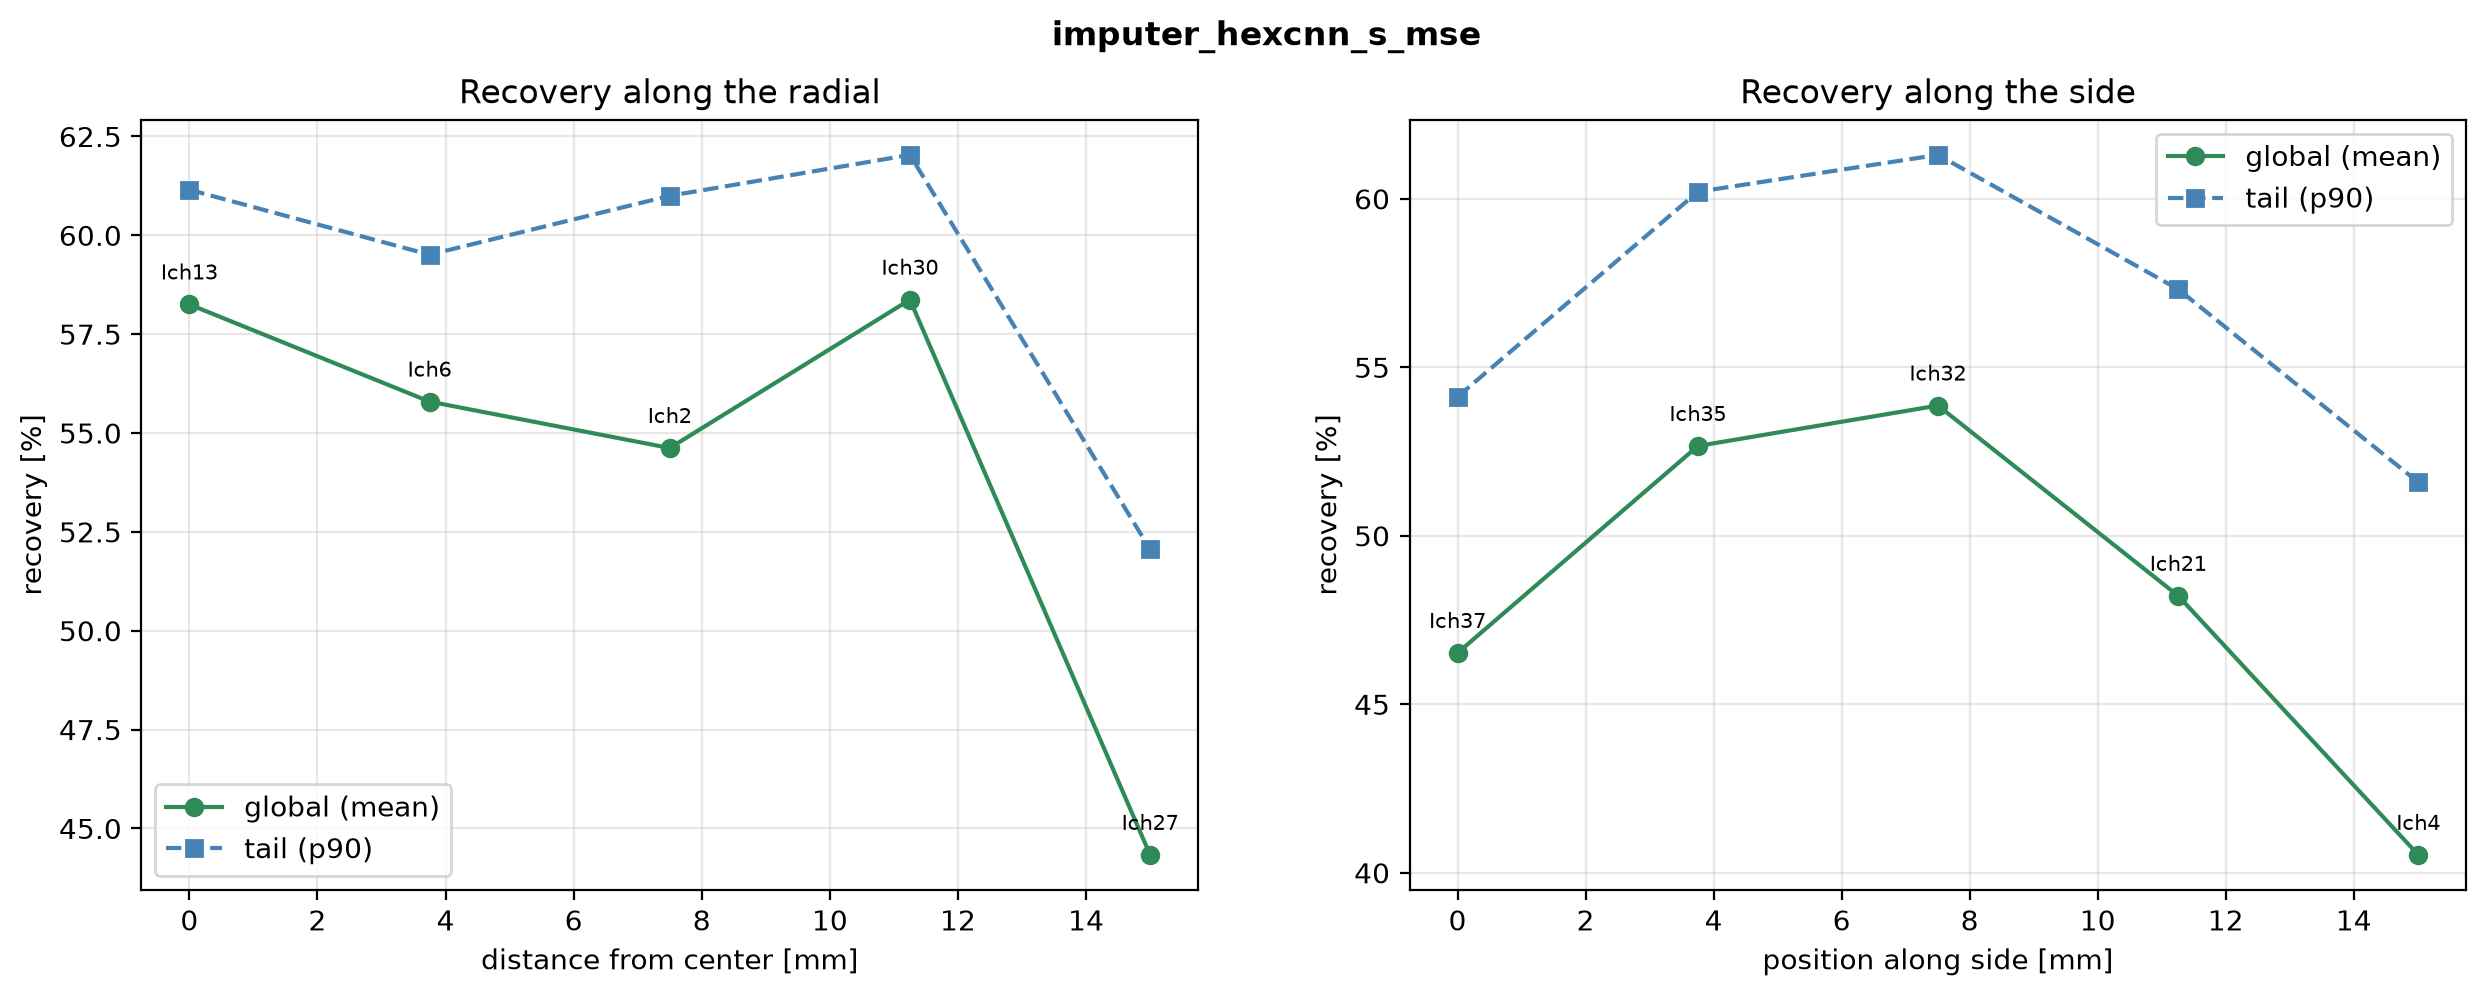
\includegraphics[width=\textwidth]{fig-perfil-lineas.png}
\caption{\textbf{Cómo varía el rendimiento del centro al borde.} En lugar de mirar los 61
sensores a la vez, se recorren dos trayectos: el \textbf{panel izquierdo} sigue una línea
radial desde el sensor central hasta un vértice, y el \textbf{derecho} recorre uno de los
lados del hexágono. En ambos, el eje horizontal es la posición a lo largo del trayecto en
milímetros y el vertical el porcentaje recuperado. La \textbf{línea verde continua} es la
recuperación media y la \textbf{línea azul discontinua} la del 10\,\% de eventos peores;
cada punto lleva la etiqueta del sensor correspondiente. La lectura es que el rendimiento se
mantiene estable en torno al 55--58\,\% en casi todo el recorrido y \textbf{cae en el último
punto}, que en ambos casos es un sensor de vértice o esquina (\texttt{Ich\,27} e
\texttt{Ich\,4}). Es coherente con que esos sensores reciben menos luz y tienen menos vecinos
de los que extraer información.}
\label{fig:perfil}
\end{figure}

\section{¿De dónde viene el rendimiento? La geometría importa}

Una pregunta razonable es si la red está usando realmente la disposición física de los
sensores o si simplemente tiene parámetros suficientes para memorizar correlaciones. El
experimento que lo resuelve es una \textbf{ablación}: se entrena exactamente la misma red,
con el mismo número de parámetros y los mismos datos, pero \textbf{barajando las etiquetas
del grafo de vecindad}. El modelo sigue creyendo que cada sensor tiene seis vecinos, pero
esos vecinos ya no son los que están físicamente al lado.

\begin{figure}[H]
\centering
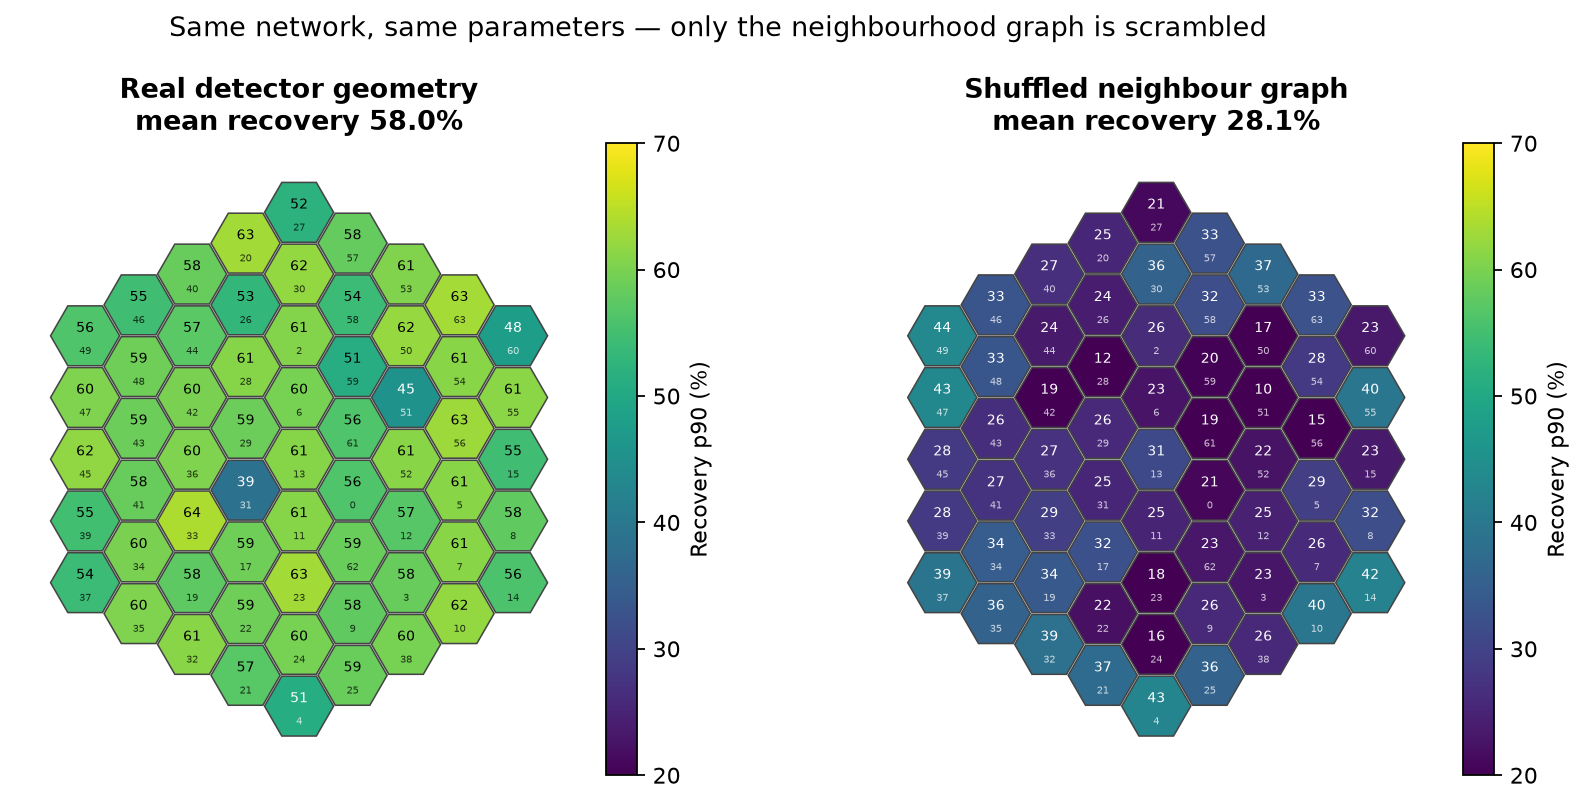
\includegraphics[width=\textwidth]{fig-ablacion.png}
\caption{\textbf{La geometría es esencial.} Ambos paneles son el mismo mapa de sensores de
la figura anterior, con la recuperación del 10\,\% de eventos peores. A la
\textbf{izquierda}, la red entrenada con la geometría real del detector: recuperación media
del \textbf{58.0\,\%}, con los hexágonos en tonos verdes y amarillos. A la
\textbf{derecha}, la misma red con el grafo de vecindad barajado: la recuperación cae al
\textbf{28.1\,\%} y el mapa se vuelve azul y morado. La escala de color es idéntica en los
dos paneles, de morado oscuro (20\,\%) a amarillo (70\,\%), de modo que la comparación es
directa. \textbf{Perder la geometría cuesta treinta puntos}, prácticamente la mitad del
rendimiento.}
\label{fig:ablacion}
\end{figure}

\subsection{¿Y hace falta una red neuronal?}

La segunda pregunta obligada es si un método clásico bastaría. Se compararon tres
procedimientos sobre exactamente los mismos eventos de prueba: promediar los vecinos
inmediatos del sensor averiado, ajustar una regresión lineal que prediga su carga a partir
de los otros sesenta, y la red. Todos ellos excluyen, por supuesto, el sensor que deben
reconstruir.

\begin{table}[H]
\centering
\caption{Comparación con métodos clásicos, sobre los mismos eventos.}
\label{tab:baselines}
\begin{tabular}{lrr}
\toprule
\textbf{Método} & \textbf{Recuperación p90} (\%) & \textbf{Error de carga} (ADC) \\
\midrule
Media de los vecinos & 45.4 & 0.891 \\
Regresión lineal (60 sensores) & 46.6 & 0.831 \\
\textbf{Red neuronal} & \textbf{58.0} & \textbf{0.619} \\
\midrule
Ventaja de la red & $+11.4$ puntos & $-25\,\%$ \\
\bottomrule
\end{tabular}
\end{table}

La regresión lineal apenas mejora al promedio de vecinos, mientras que la red saca once
puntos a ambas. La relación entre la carga de un sensor y la de sus vecinos es, por tanto,
\textbf{claramente no lineal}, y ahí es donde el aprendizaje profundo aporta.

Un experimento complementario refuerza el diseño elegido: si en lugar de usar los sesenta
sensores se ajusta la regresión usando solo los vecinos a uno, dos o tres pasos de
distancia, el rendimiento \textbf{satura ya en el segundo anillo}. Añadir sensores más
lejanos no aporta nada. Esto confirma que el problema es local y justifica una arquitectura
que solo mira a los vecinos.

\section{Los tres flancos físicos}

Recuperar la posición no basta: hay que comprobar que la reconstrucción no estropea las
otras magnitudes que el detector debe medir. Se examinaron tres.

\subsection{Energía: el espectro se conserva}

Sumando la carga de todos los sensores se obtiene la energía del evento, y su histograma
debe reproducir el espectro de la fuente de $^{22}$Na empleada. Si la reconstrucción
sistemáticamente subestimara o sobreestimara, el espectro se desplazaría y la calibración
en energía quedaría inservible.

\begin{figure}[H]
\centering
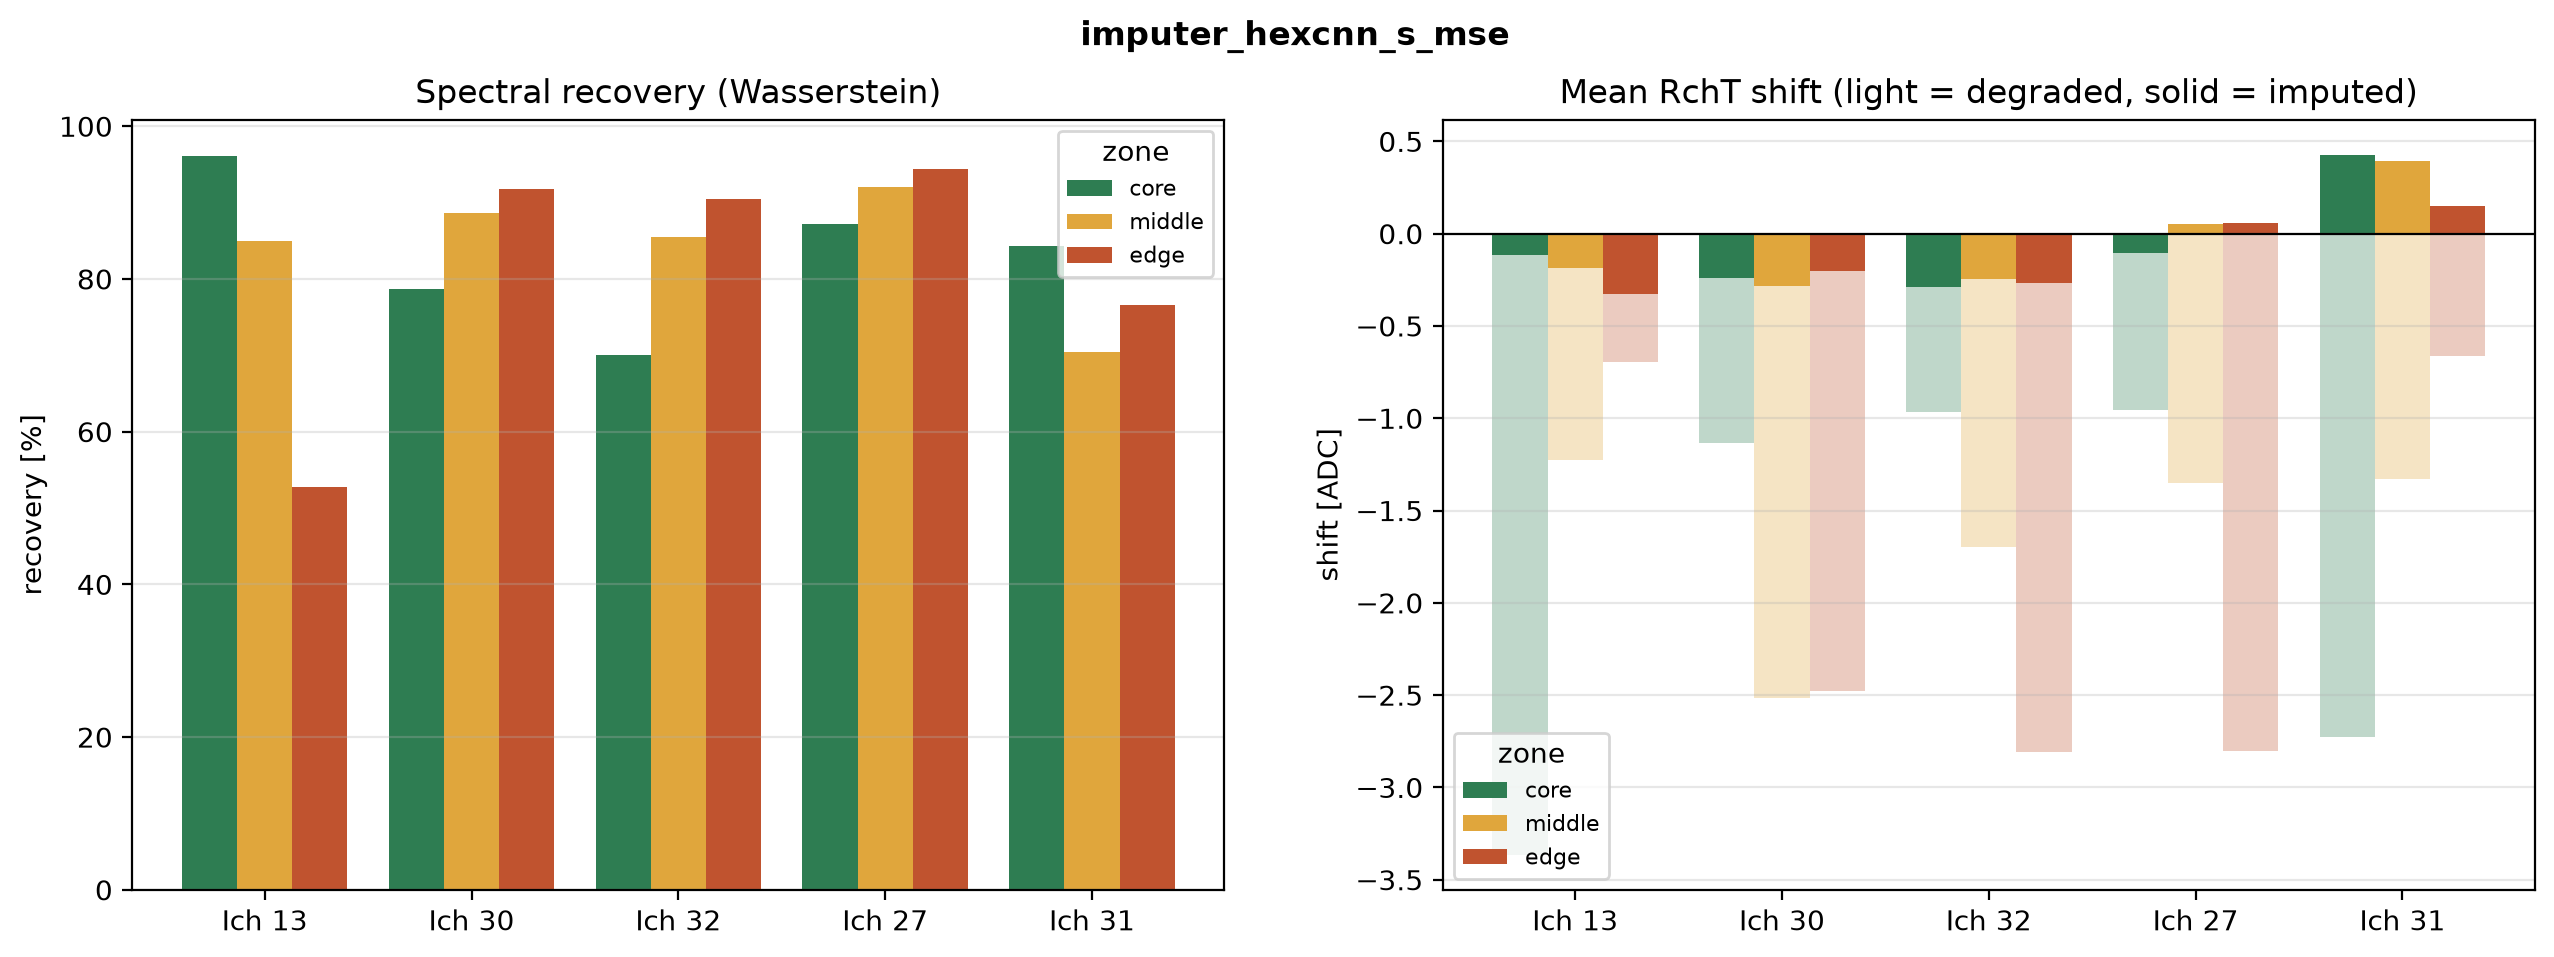
\includegraphics[width=\textwidth]{fig-espectro.png}
\caption{\textbf{Conservación del espectro de energía.} El análisis se estratifica en tres
zonas del detector según dónde ocurrió el evento: \textbf{verde} para el núcleo, \textbf{amarillo}
para la corona intermedia y \textbf{rojo} para el borde. En el \textbf{panel izquierdo}, la
altura de cada barra es el porcentaje del daño espectral que se repara, para cinco sensores
averiados distintos; casi todas las barras superan el 80\,\%, con una media del 82.9\,\%. En
el \textbf{panel derecho} se muestra el desplazamiento de la energía media en unidades ADC:
las \textbf{barras claras y largas} son el desplazamiento que provoca el fallo sin corregir,
y las \textbf{barras sólidas y cortas} el que queda tras la reconstrucción. La lectura es
inmediata: \textbf{las barras sólidas son mucho más cortas que las claras}, es decir, la
mayor parte del desplazamiento se elimina. El único caso flojo es el sensor
\texttt{Ich\,13} evaluado sobre eventos de borde (barra roja del primer grupo, 52.8\,\%),
que corresponde a reconstruir el sensor central cuando el evento ocurrió en una esquina.}
\label{fig:espectro}
\end{figure}

\subsection{Resolución espacial: la imagen se afila}

El desplazamiento medio no lo dice todo. Un fallo no solo mueve la posición reconstruida:
también la \emph{emborrona}. Conviene por tanto separar las dos componentes, el sesgo (que
la nube de puntos se desplace) y la dispersión (que se ensanche).

\begin{figure}[H]
\centering
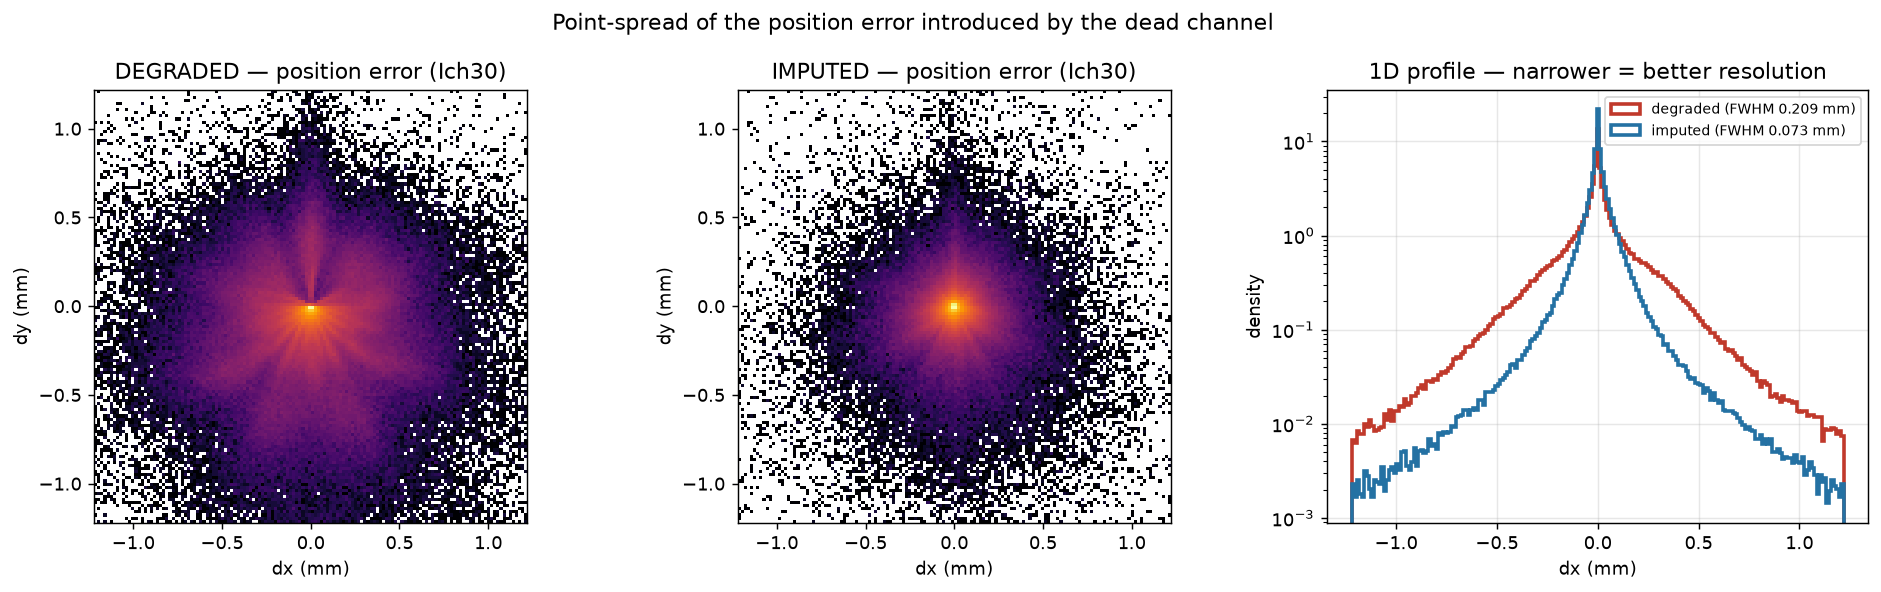
\includegraphics[width=\textwidth]{fig-resolucion.png}
\caption{\textbf{Descomposición del error en sesgo y emborronamiento.} Los dos primeros
paneles son histogramas bidimensionales del error de posición: cada punto representa la
diferencia entre la posición reconstruida y la verdadera, en milímetros, de modo que el
centro exacto significa error nulo y el color indica cuántos eventos caen en cada píxel,
del negro (ninguno) al amarillo (máximo). El \textbf{panel izquierdo} corresponde al sensor
averiado sin corregir y el \textbf{central} a la situación tras la reconstrucción: la nube
es visiblemente \textbf{más compacta y está mejor centrada}. El \textbf{panel derecho}
superpone los perfiles unidimensionales de ambas distribuciones: la \textbf{curva roja} es
el caso degradado y la \textbf{curva azul} el reconstruido. La curva azul es
\textbf{claramente más estrecha}, y su anchura a media altura pasa de 0.209 a
\SI{0.073}{\milli\metre} para este sensor. Agregando sobre los 61 sensores, la red elimina
el \textbf{48.8\,\%} del emborronamiento y el \textbf{82.7\,\%} del sesgo.}
\label{fig:resolucion}
\end{figure}

\subsection{Carga: cuánto se equivoca en la magnitud primaria}

Por último, cabe preguntarse cuánto se equivoca la red al estimar la carga en sí, que es lo
que realmente predice. Expresado en términos relativos, el error es de aproximadamente el
\textbf{30\,\%} de la carga típica del sensor.

\begin{figure}[H]
\centering
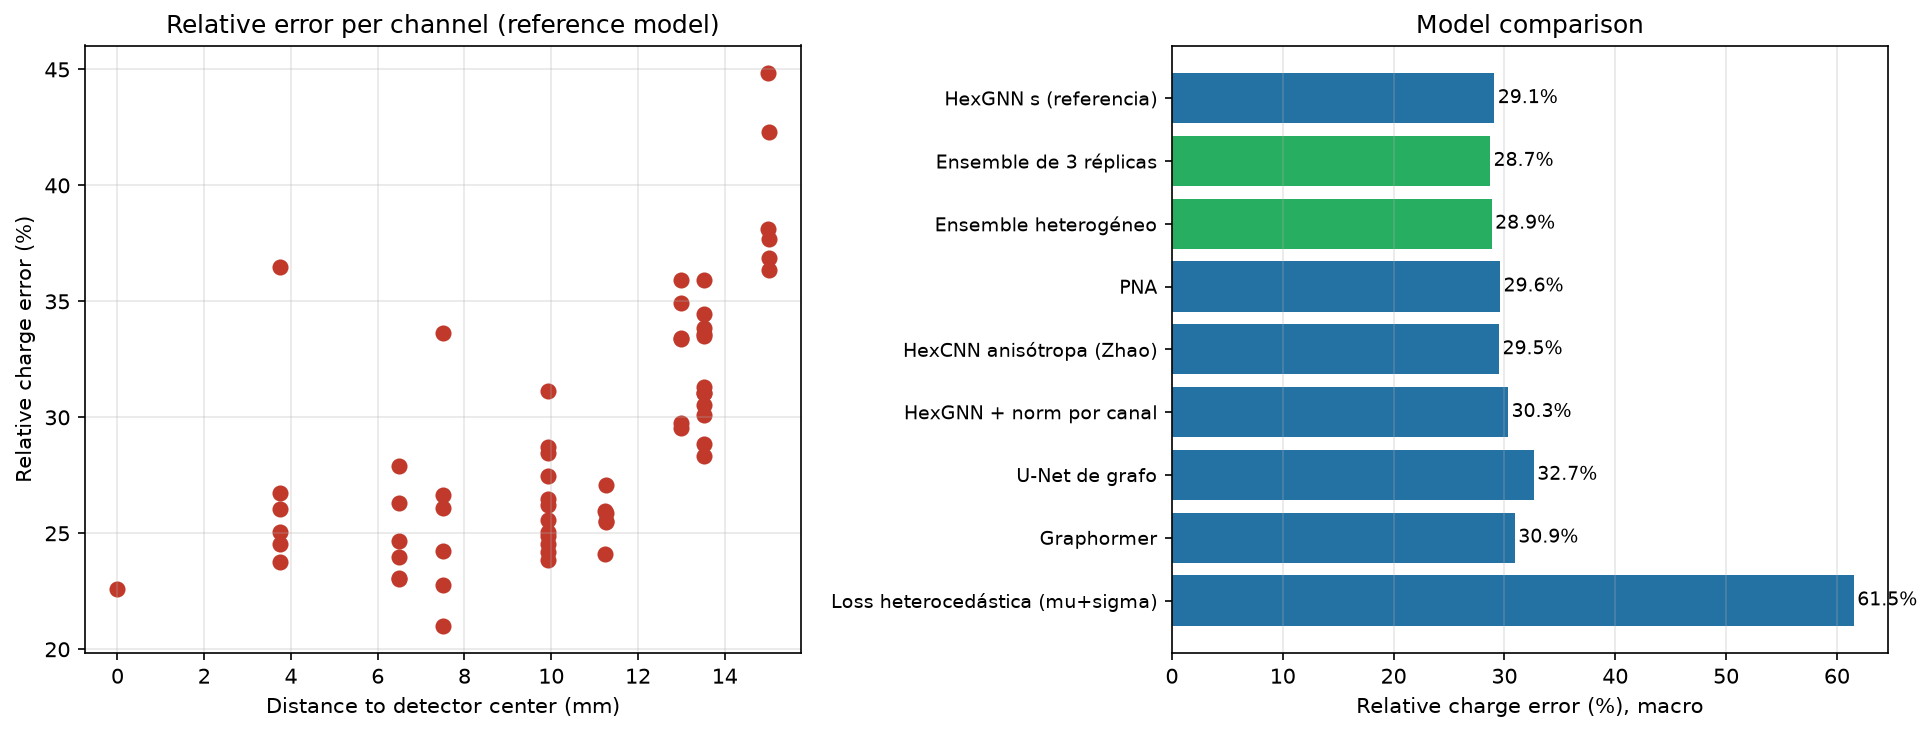
\includegraphics[width=\textwidth]{fig-error-relativo.png}
\caption{\textbf{Error relativo de carga.} En el \textbf{panel izquierdo}, cada punto rojo
es uno de los 61 sensores, situado según su distancia al centro del detector; el eje
vertical es el error relativo con que se reconstruye su carga. Se aprecia una
\textbf{tendencia creciente clara}: los sensores del centro se reconstruyen con un error en
torno al 25\,\% y los del borde superan el 35\,\%, lo que enlaza con el gradiente de
iluminación de la Figura~\ref{fig:detector}. El \textbf{panel derecho} compara el error
relativo medio de las distintas configuraciones ensayadas; las \textbf{barras verdes} son
los dos \emph{ensembles} y las \textbf{azules} el resto. Todas las variantes razonables se
agrupan entre el 29 y el 33\,\%, salvo la última ---un intento de que la red estimase su
propia incertidumbre--- que se dispara al 61.5\,\% y se descartó.}
\label{fig:errorrelativo}
\end{figure}

\begin{idea}
\noindent\textbf{Una observación que merece destacarse.} Un error del 30\,\% en la carga de
un sensor se traduce en apenas \SI{0.13}{\milli\metre} de error en la posición. La razón es
que el centro de gravedad promedia sobre 61 sensores, de modo que un error grande en uno
solo queda muy diluido. Esto explica por qué el método funciona bien en posición aunque la
estimación de carga individual sea modesta, y es el argumento físico que justifica el
enfoque.
\end{idea}

\section{Cuando falla más de un sensor}

En los módulos reales los fallos no siempre son de un único sensor. A veces se estropea un
grupo contiguo ---por una sombra, una conexión en serie o un efecto térmico--- y a veces
aparecen varios sensores afectados a poca distancia unos de otros. Se estudiaron por tanto
dos regímenes: \textbf{contiguo}, en el que los sensores averiados forman un grupo compacto,
y \textbf{disperso}, en el que se reparten por el detector y que sirve de control.

\begin{figure}[H]
\centering
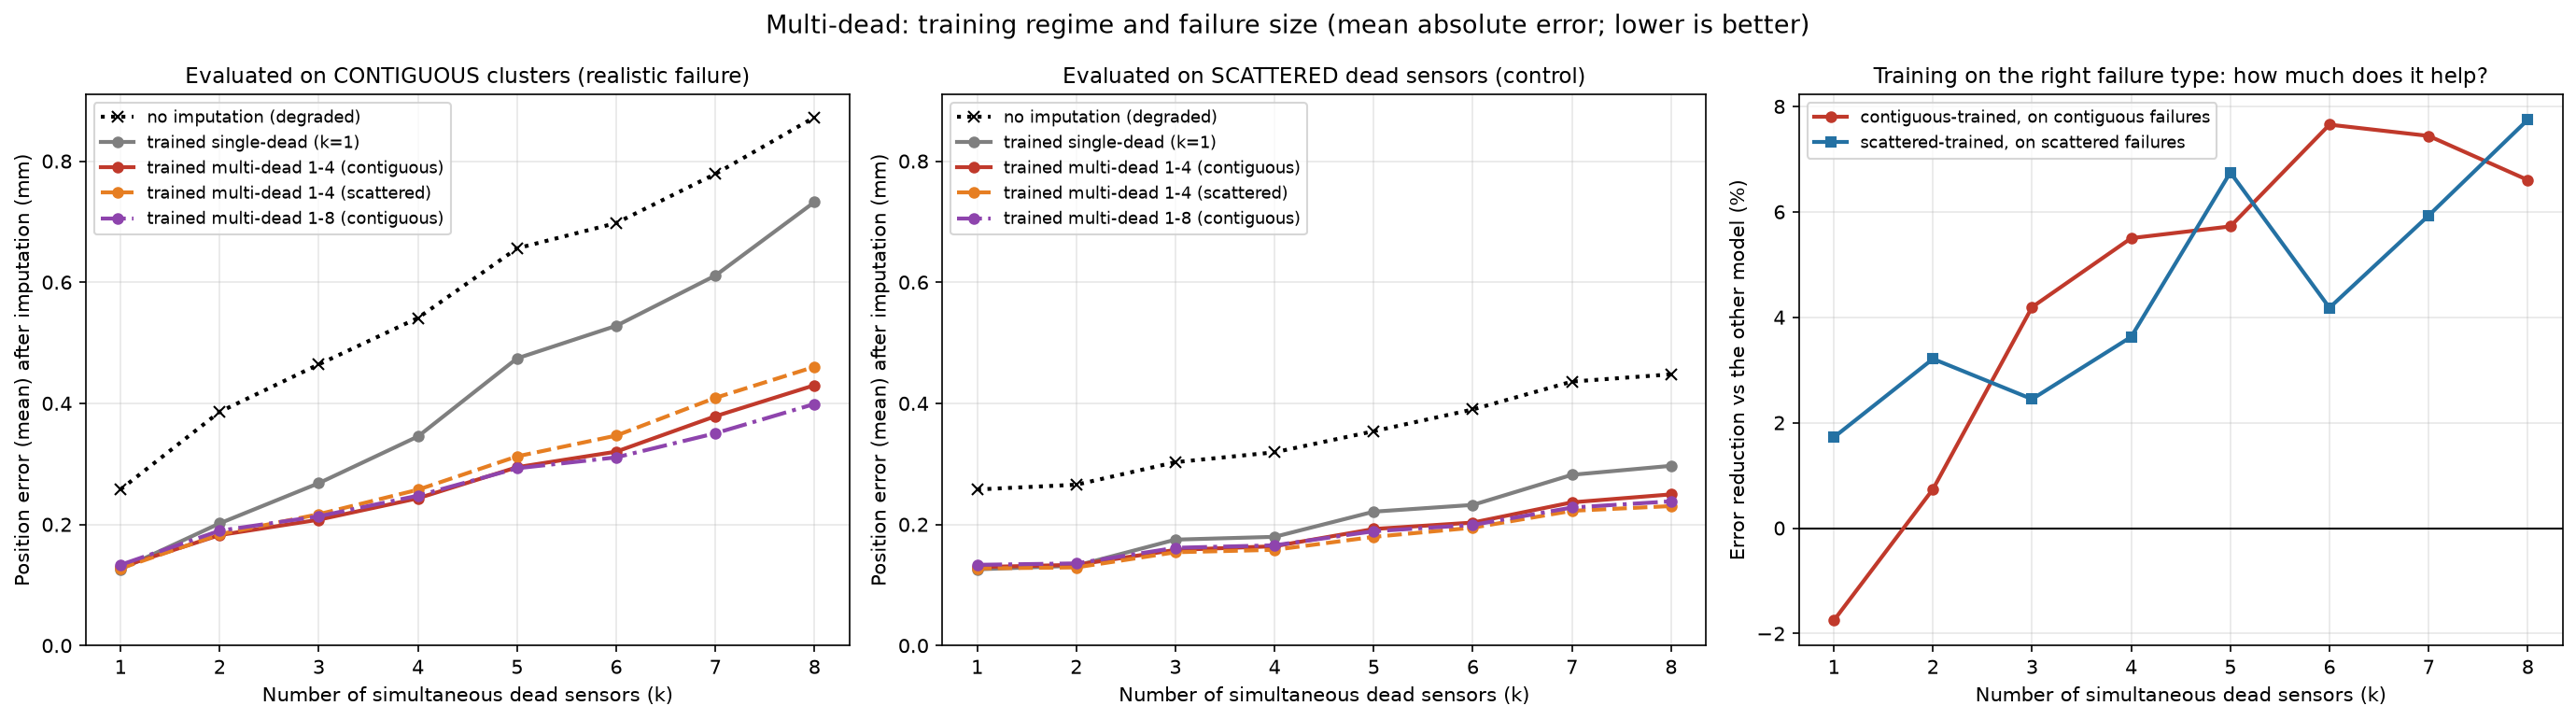
\includegraphics[width=\textwidth]{fig-multidead.png}
\caption{\textbf{Comportamiento frente al tamaño del fallo.} En los dos primeros paneles el
eje horizontal es el número de sensores averiados simultáneamente, de uno a ocho, y el
vertical el error de posición que queda tras la reconstrucción en milímetros, de modo que
\textbf{más abajo es mejor}. El \textbf{panel izquierdo} evalúa grupos contiguos, el caso
físicamente realista, y el \textbf{central} sensores dispersos, como control. En ambos, la
\textbf{línea negra de puntos} es la situación sin reconstruir, es decir, el daño que causa
el fallo. La \textbf{línea gris} corresponde al modelo entrenado únicamente con un sensor
apagado, y se ve cómo \textbf{se despega hacia arriba} a partir de cuatro o cinco sensores:
fuera de aquello para lo que fue entrenado, se degrada deprisa. Las líneas
\textbf{roja} (entrenada con grupos contiguos de uno a cuatro), \textbf{naranja} (dispersos)
y \textbf{morada} (contiguos de uno a ocho) se mantienen \textbf{muy por debajo}, cerca de la
mitad del error, incluso con ocho sensores caídos. El \textbf{panel derecho} cuantifica
cuánto se gana entrenando con el tipo de fallo correcto: la \textbf{línea roja} indica la
mejora del modelo entrenado en contiguo al evaluarse en fallos contiguos y la \textbf{azul}
la del entrenado en disperso sobre fallos dispersos; ambas son positivas a partir de dos
sensores, de modo que \textbf{conviene entrenar con el modo de fallo que se espera
encontrar}.}
\label{fig:multidead}
\end{figure}

La conclusión práctica es que \textbf{entrenar con varios sensores apagados sale
esencialmente gratis}: con un solo fallo el modelo rinde igual que el especializado, y a
cambio aguanta mucho mejor los fallos grandes, incluso los de tamaño superior a los vistos
durante el entrenamiento.

\subsection{Con qué tipo de avería conviene entrenar}

Queda una pregunta más fina, y su respuesta resultó ser el hallazgo más aprovechable de las
últimas sesiones. Los dos regímenes anteriores ---sensores pegados y sensores repartidos por
todo el detector--- son los dos \emph{extremos}. Al revisar a mano los módulos averiados
reales aparece, sin embargo, un tercer caso muy frecuente que no estaba representado:
\textbf{dos o tres sensores separados por una o dos posiciones}, ni pegados ni lejanos. Se
añadió por ello un régimen intermedio, y se comprobó que efectivamente ocupa el punto medio:
la separación media entre los sensores averiados es de 1.8 posiciones, frente a 1.2 en el
contiguo y 17.6 en el disperso.

\begin{figure}[H]
\centering
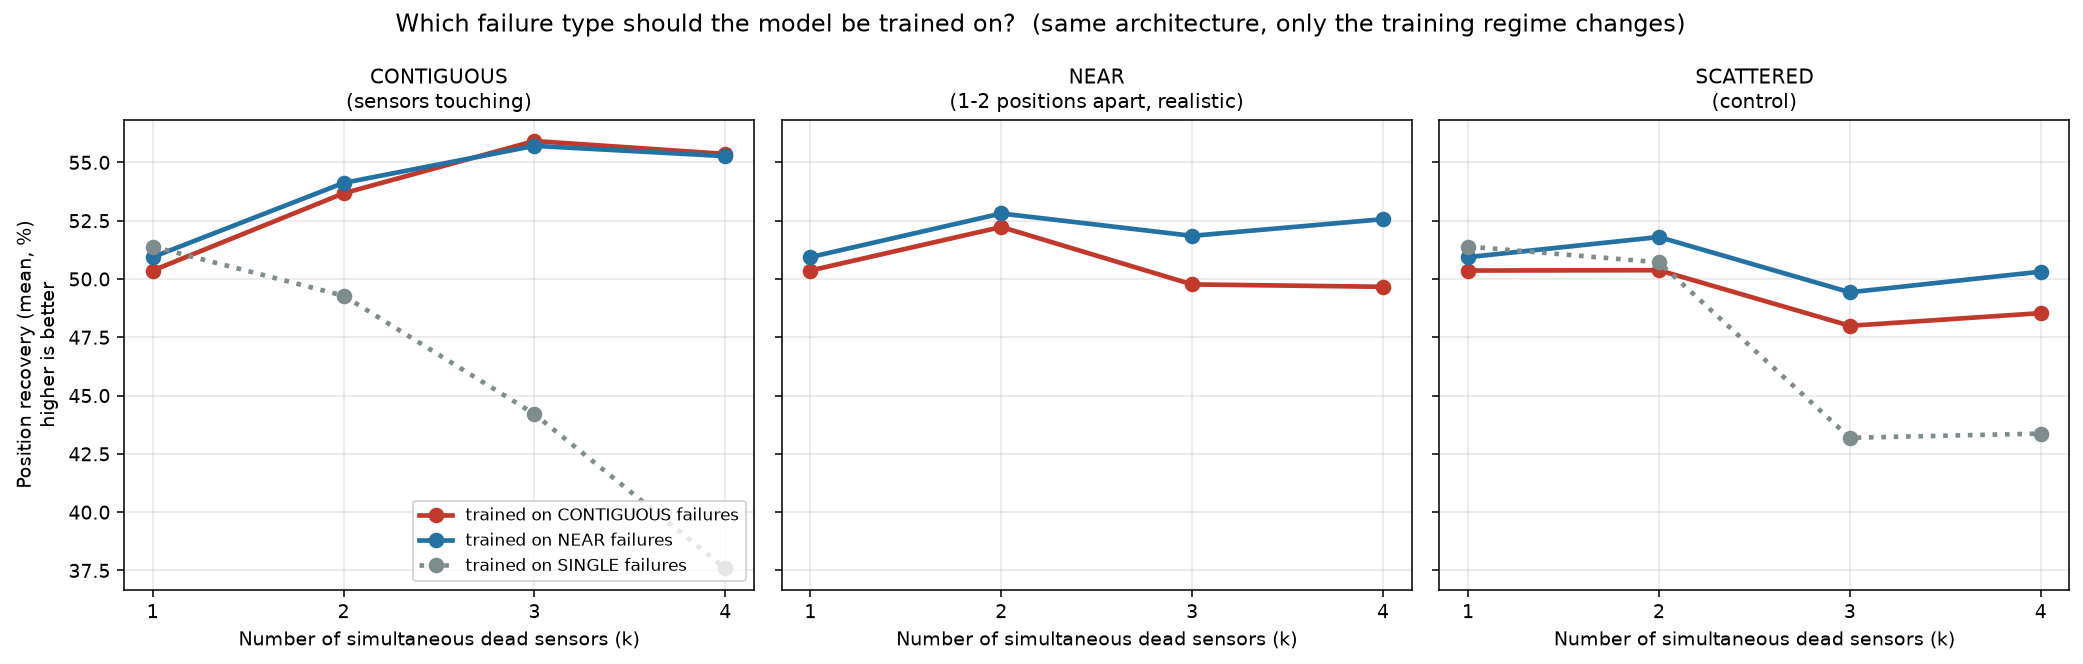
\includegraphics[width=\textwidth]{fig-regimenes.png}
\caption{\textbf{Con qué tipo de avería conviene entrenar el modelo.} Los tres paneles
corresponden a los tres tipos de fallo sobre los que se \emph{evalúa}: sensores contiguos a
la izquierda, el caso realista intermedio en el centro, y sensores dispersos a la derecha.
Dentro de cada panel, el eje horizontal es el número de sensores averiados y el vertical el
porcentaje de posición recuperada, de modo que \textbf{más arriba es mejor}. Las tres curvas
son el \emph{mismo modelo} entrenado de tres maneras distintas: la \textbf{línea gris de
puntos} entrenada con un solo sensor averiado, la \textbf{roja} con grupos contiguos y la
\textbf{azul} con el caso intermedio. La lectura es directa: en el panel izquierdo la roja y
la azul \textbf{se superponen} ---entrenar con el caso intermedio no cuesta nada frente a
entrenar con contiguos---, mientras que en los paneles central y derecho \textbf{la azul
queda por encima}, hasta casi tres puntos. La gris se desploma en cuanto falla más de un
sensor, que es el peaje de no haber entrenado nunca con averías múltiples.}
\label{fig:regimenes}
\end{figure}

La interpretación es geométrica y se sostiene sin necesidad de más experimentos: el régimen
intermedio ocupa una posición central en el espacio de configuraciones de avería, de manera
que \textbf{entrenar en el punto medio generaliza hacia los dos extremos, mientras que
entrenar en un extremo no alcanza el centro}. La consecuencia práctica es que el modelo
destinado a producción debería entrenarse con este régimen, que además es el que corresponde
a lo que realmente se observa en los módulos averiados.

\section{Cuánto varía de un detector a otro}
\label{sec:variabilidad}

Este es el resultado metodológicamente más relevante de las últimas semanas y conviene
detenerse en él, porque cambia cómo deben leerse todas las cifras anteriores.

Las métricas se calculan sobre cinco módulos reservados para prueba. Cinco es una muestra
holgada en número de eventos ---varios millones--- pero pobre en número de
\emph{detectores}. La pregunta natural es cuánto dependen los resultados de qué cinco
módulos concretos tocaron.

Existe una forma barata de responderla. Por el modo en que se cargan los datos, el modelo de
referencia solo llega a ver 40 de los 149 módulos de entrenamiento; los demás nunca los ha
observado y son, a efectos prácticos, un conjunto de prueba adicional de gran tamaño.

\begin{figure}[H]
\centering
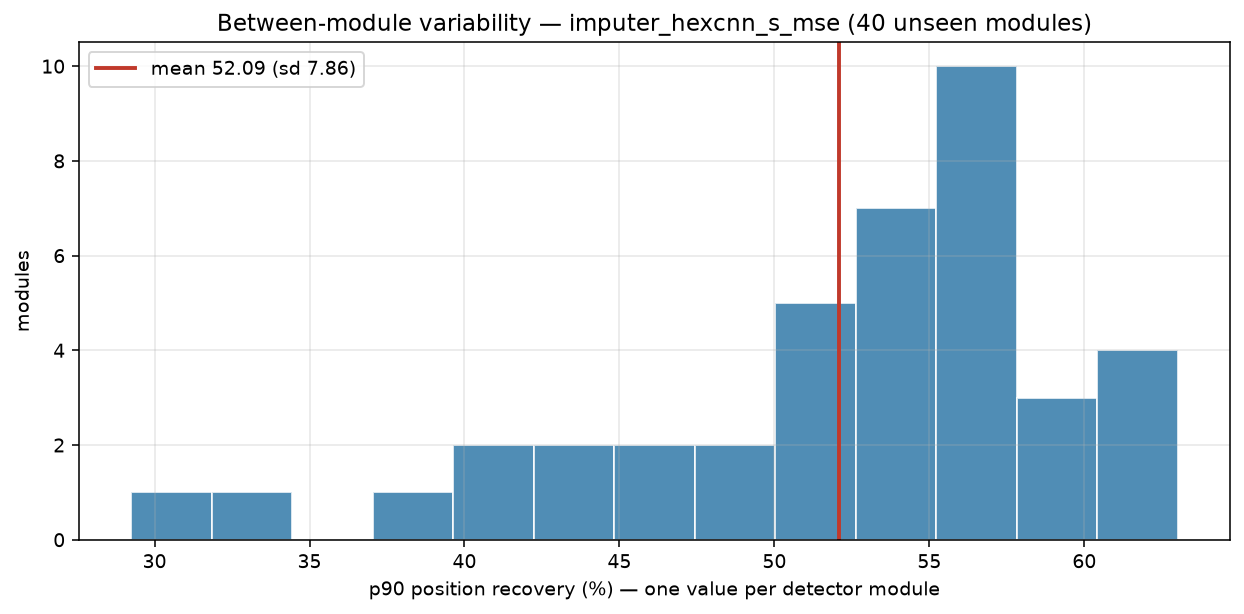
\includegraphics[width=0.85\textwidth]{fig-variabilidad-modulos.png}
\caption{\textbf{Variabilidad entre detectores.} Histograma del rendimiento del \emph{mismo}
modelo evaluado sobre 40 módulos que nunca vio durante el entrenamiento. Cada
\textbf{barra azul} agrupa los módulos cuyo porcentaje de recuperación cae en ese intervalo,
y su altura es cuántos módulos hay. La \textbf{línea roja vertical} marca la media, situada
en el 52.1\,\%. Lo llamativo es \textbf{la anchura de la distribución}: hay módulos en los
que la recuperación no llega al 30\,\% y otros en los que supera el 63\,\%, con una
desviación típica de \textbf{7.9 puntos}. Es decir, el mismo modelo, aplicado a detectores
distintos, da resultados muy distintos.}
\label{fig:variabilidad}
\end{figure}

Para poner esa cifra en contexto: repitiendo el mismo entrenamiento cuatro veces con distinta
semilla de inicialización, la dispersión de los resultados es de apenas \textbf{0.13
puntos}. La variabilidad debida a \textbf{qué detector} se mide es, por tanto, unas
\textbf{sesenta veces mayor} que la debida a cómo se entrenó.

\subsection{La comprobación definitiva: repetirlo todo cinco veces}

El análisis anterior mide la variabilidad de la \emph{medida}. Queda una pregunta más
exigente: si se rehiciera el trabajo entero ---partición, entrenamiento y evaluación---
reservando otros cinco detectores, ¿saldría lo mismo? Para responderla se repitió el
procedimiento completo con \textbf{cinco particiones independientes}.

\begin{table}[H]
\centering
\caption{El procedimiento completo repetido con cinco particiones distintas de los datos.
Cada fila reserva cinco detectores diferentes para la evaluación final.}
\label{tab:cv}
\begin{tabular}{lrrr}
\toprule
\textbf{Partición} & \textbf{Recuperación p90} (\%) & \textbf{Recuperación media} (\%) &
\textbf{Error de carga} \\
\midrule
A (la empleada hasta ahora) & 58.07 & 52.60 & 0.619 \\
B & 58.22 & 51.97 & 0.629 \\
C & 55.46 & 49.88 & 0.644 \\
D & 52.98 & 47.35 & 0.686 \\
E & 58.30 & 52.30 & 0.610 \\
\midrule
\textbf{Media $\pm$ desviación} & $\mathbf{56.6 \pm 2.3}$ & $\mathbf{50.8 \pm 2.2}$ &
$0.637 \pm 0.030$ \\
\bottomrule
\end{tabular}
\end{table}

El recorrido entre la mejor y la peor partición es de \textbf{5.3 puntos}, superior a
cualquier diferencia entre modelos reportada en todo el trabajo. Y conviene señalar que la
partición empleada durante el desarrollo resultó ser de las favorables.

\begin{idea}
\noindent\textbf{Qué cambia y qué no.} Este es probablemente el punto más importante del
informe, y es fácil sacar la conclusión equivocada.

\smallskip
\noindent\textbf{Lo que no cambia:} todas las comparaciones entre modelos siguen siendo
válidas. Se hacen sobre \emph{los mismos} detectores para todos los modelos, de modo que el
efecto de la partición se cancela al restar. Ninguna conclusión del trabajo se ve afectada.

\smallskip
\noindent\textbf{Lo que sí cambia:} la cifra absoluta. No puede afirmarse que el método
recupere el 58\,\% en un detector cualquiera; lo correcto es $\mathbf{56.6 \pm 2.3\,\%}$, y
la dispersión entre unidades individuales llega a $\pm 7.9$ puntos.

\smallskip
\noindent Es la distinción entre \emph{precisión relativa} ---excelente: se pueden ordenar
modelos con confianza--- y \emph{exactitud absoluta} ---mucho más incierta: no se sabe con
precisión qué rendimiento tendría en un equipo nuevo---. Ambas cosas son ciertas a la vez.
\end{idea}

Este resultado explicó además un caso que llevaba semanas abierto. El sensor
\texttt{Ich\,31} aparecía como el peor del detector en la Figura~\ref{fig:mapa}, con un
39\,\% frente al 58\,\% típico, y se sospechaba que era un fotosensor defectuoso. Resultó
que dos de los cinco módulos de prueba tienen una respuesta muy alejada de la que el modelo
había visto al entrenar. Al reentrenar cubriendo los 149 módulos, ese sensor
\textbf{sube de 38.6 a 49.5\,\%}. No era un sensor malo: era un sensor que la red no sabía
tratar porque nunca había visto detectores parecidos.

\section{Detección automática de sensores averiados}

Todo lo anterior presupone saber qué sensor está estropeado. En los módulos reales esa
información no viene dada, así que se desarrolló un procedimiento para identificarlos. La
dificultad está en la Figura~\ref{fig:detector}: un umbral único no sirve, porque un sensor
de esquina sano se activa menos que un sensor central averiado. El criterio compara por
tanto cada sensor \textbf{con lo que se espera de un sensor en su misma posición},
estimado sobre los módulos sanos.

\begin{figure}[H]
\centering
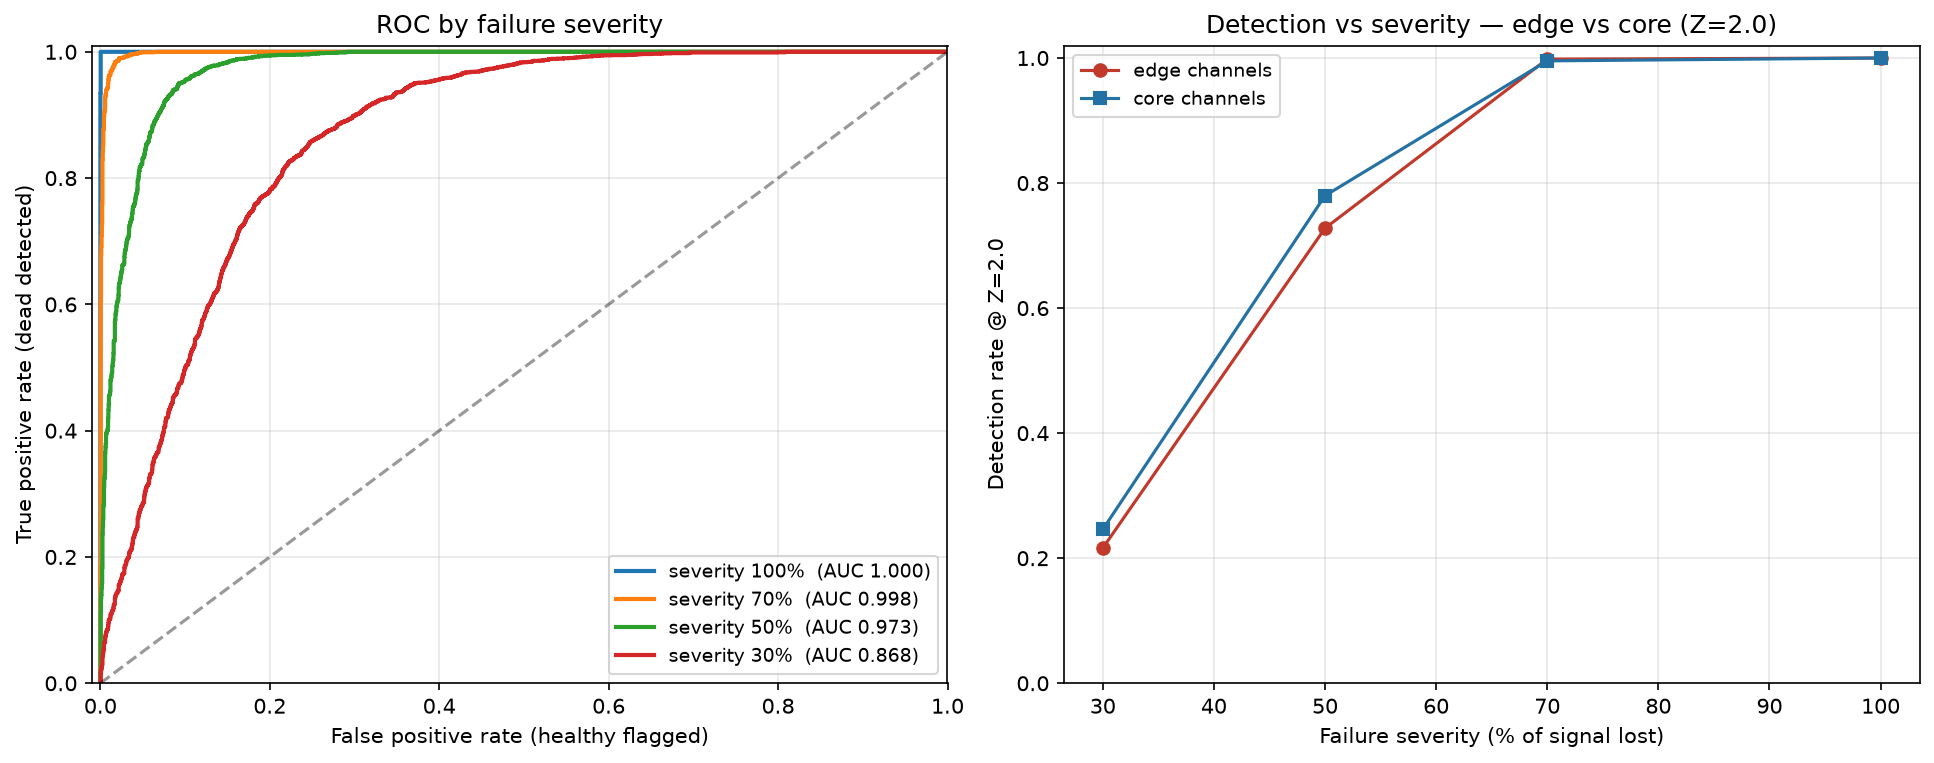
\includegraphics[width=\textwidth]{fig-deteccion-roc.png}
\caption{\textbf{Validación del detector de sensores averiados.} Como en los módulos reales
no hay diagnóstico de referencia, se degradaron artificialmente sensores de módulos sanos
para tener una verdad conocida. El \textbf{panel izquierdo} muestra las curvas ROC: el eje
horizontal es la fracción de sensores sanos marcados por error y el vertical la fracción de
averiados correctamente detectados, de modo que \textbf{cuanto más pegada a la esquina
superior izquierda, mejor}. Cada color corresponde a una severidad del fallo: la
\textbf{curva azul} es un sensor completamente muerto, la \textbf{naranja} uno que perdió el
70\,\% de su señal, la \textbf{verde} el 50\,\% y la \textbf{roja} el 30\,\%. La curva azul
llega prácticamente al vértice, con área bajo la curva igual a \textbf{1.000}: los sensores
muertos se detectan sin ambigüedad. La degradación se va notando conforme el fallo es más
sutil, hasta 0.868 para el caso del 30\,\%. El \textbf{panel derecho} comprueba que el
criterio no penaliza a los sensores de borde: la \textbf{línea roja} corresponde a los
sensores periféricos y la \textbf{azul} a los centrales, y ambas prácticamente se
superponen, lo que confirma que la corrección por posición funciona.}
\label{fig:roc}
\end{figure}

Aplicado a los 62 módulos averiados reales, el procedimiento señala sensores defectuosos en
48 de ellos, marcando 278 canales en total. Conviene ser explícito sobre sus límites: el
método identifica con fiabilidad los sensores completamente inactivos, pero no separa las
degradaciones moderadas del comportamiento normal, ni detecta sensores con ganancia
anómalamente \emph{alta}. El etiquetado manual de los módulos, actualmente en curso,
confirma además que la casuística real es más variada de lo que el modelo estadístico
contempla: hay fallos de un solo sensor, grupos contiguos y también conjuntos de dos o tres
sensores separados por una o dos posiciones.

\section{El techo de rendimiento: nueve intentos de superarlo}

La pregunta que ha ocupado la mayor parte del esfuerzo experimental es si ese 52\,\% de
recuperación media puede mejorarse. La respuesta, tras una campaña sistemática, es que
\textbf{no con los datos disponibles}. La Tabla~\ref{tab:techo} resume las estrategias
ensayadas.

\begin{table}[H]
\centering
\caption{Estrategias ensayadas para superar el rendimiento del modelo de referencia. La
banda de incertidumbre entre entrenamientos idénticos es de $\pm 0.35$ puntos en
recuperación media, de modo que solo diferencias mayores son interpretables.}
\label{tab:techo}
\small
\begin{tabular}{lp{8.4cm}}
\toprule
\textbf{Estrategia} & \textbf{Resultado} \\
\midrule
Aumentar el tamaño de la red & Sin mejora en media (6 y 10 veces más parámetros dan lo
mismo), aunque sí mejora el peor sensor \\
Términos físicos en la función de coste & El de posición resulta redundante; el de energía
empeora claramente \\
Geometría métrica (distancias y direcciones) & Efecto nulo: el problema es isótropo \\
Atención global entre todos los sensores & Peor de forma reproducible: el problema es local \\
Arquitecturas del estado del arte (\emph{transformer}, U-Net de grafo) & Mejores en
validación pero iguales o peores en prueba \\
Convolución hexagonal direccional & Empate exacto \\
Normalizaciones alternativas & Sin mejora o peor \\
Cobertura completa de módulos & Sin efecto en la media; mejora la homogeneidad \\
Mezclar módulos dentro de cada lote & Sin efecto \\
\midrule
\textbf{Promediar varios modelos} & \textbf{Única mejora real: entre 1.7 y 2.5 puntos,
a costa de triplicar el coste de inferencia} \\
\bottomrule
\end{tabular}
\end{table}

Que nueve estrategias independientes converjan al mismo valor es, en sí mismo, el resultado
más sólido del trabajo. Y hay un argumento adicional que lo refuerza: promediar tres modelos
entrenados por separado ---que es la forma habitual de estimar cuánta parte del error se
debe a la variabilidad del ajuste y cuánta es irreducible--- solo reduce el error un 2\,\%.
Es decir, \textbf{el 98\,\% del error restante no procede del modelo}, sino de que la
información necesaria sencillamente no está presente en los sensores supervivientes.

\begin{idea}
\noindent\textbf{Conclusión central.} El aprendizaje profundo es necesario, porque supera en
once puntos a los métodos clásicos y la relación es marcadamente no lineal. La geometría es
necesaria, porque prescindir de ella cuesta treinta puntos. Pero una vez incorporadas ambas,
\textbf{una red pequeña de 38\,000 parámetros satura el problema}. El límite no está en la
arquitectura: está en la física.
\end{idea}

\section{Estado actual y decisiones abiertas}

El método funciona y está caracterizado en sus tres flancos físicos. Quedan tres cuestiones
sobre las que conviene decidir.

La primera es \textbf{qué configuración adoptar como modelo de producción}, y la respuesta
depende del modo de fallo que se espere. Si lo habitual son sensores aislados, la versión
entrenada con cobertura completa es preferible porque responde de forma más homogénea: su
peor sensor rinde un 47.8\,\% frente al 39.4\,\% de la referencia. Si se esperan grupos
contiguos, conviene la versión entrenada en régimen múltiple. Ambas mejoras no se acumulan
tan bien como cabría esperar, y ahí queda trabajo por hacer.

La segunda es la \textbf{calibración en energía}, que no se ha aplicado. Todas las
conclusiones se sostienen sin ella porque el diseño de la evaluación es diferencial y los
efectos de calibración se cancelan, pero no puede descartarse que un conjunto calibrado
permitiera superar el límite observado.

La tercera es la \textbf{validación sobre módulos averiados reales}. Hasta ahora el detector
de sensores defectuosos se ha validado con fallos inyectados artificialmente, que garantizan
una verdad conocida a costa de representar un modo de fallo idealizado. El etiquetado manual
en curso proporcionará la referencia necesaria para medir el acuerdo con el procedimiento
automático sobre datos reales.

\vfill
\begin{center}
\rule{0.4\textwidth}{0.4pt}\\[0.3cm]
\small Las figuras de este informe proceden de las evaluaciones documentadas en el
repositorio del proyecto. Todas las comparaciones entre modelos se han realizado sobre los
mismos módulos de prueba y con el mismo número de eventos.
\end{center}

\end{document}
